\subsection{Sensitivity to Observation Quality}
\label{sec:robustness}

\begin{figure*}[t]
\centering
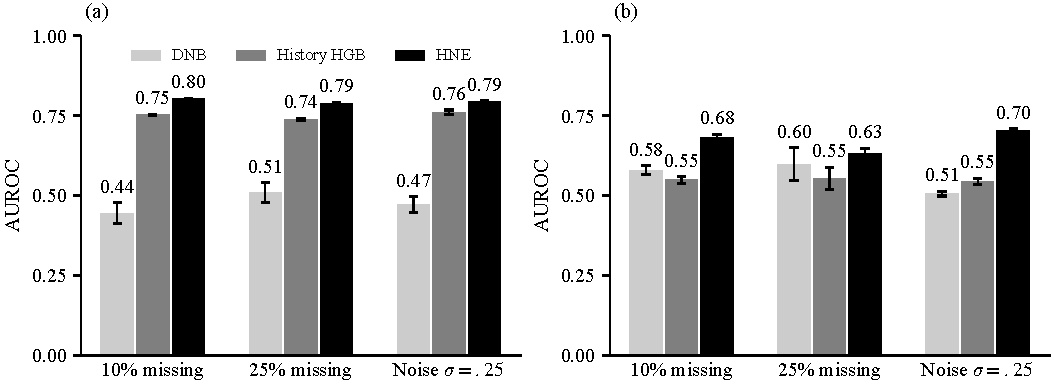
\includegraphics[width=\textwidth]{figures/robustness.pdf}
\caption{Observation perturbations: (a) RESILIENT; (b) BrisT1D-Open. Bars average three seeds, with seed standard deviations. All methods score common origins.}
\label{fig:robustness}
\end{figure*}




We perturb observed histories while holding the reference, future labels, and fitted models fixed. Figure~\ref{fig:robustness} compares HNE, History HGB, and DNB under 10\% or 25\% additional missingness and Gaussian noise of standard deviation $0.25$, averaging three seeds on common scoreable origins.

With 25\% additional missingness, HNE reaches AUROC $0.788$ on RESILIENT and $0.632$ on BrisT1D; under added noise, it reaches $0.795$ and $0.704$, respectively. BrisT1D is more sensitive to lost observations, while HNE retains the highest score among the three methods in each condition. Appendix~\ref{app:additional-results} reports all conditions; common-origin coverage at 25\% removal is 1,727--1,756 for RESILIENT and 1,195--1,206 for BrisT1D.
